\documentclass[aspectratio = 1609]{beamer}
\beamertemplatenavigationsymbolsempty

\pdfstringdefDisableCommands{\def\translate{}}

%\usepackage[latin1]{inputenc}
\usepackage{amsmath, mathtools}
\usepackage{amsfonts}
\usepackage{amssymb,stmaryrd}
\usepackage{amsthm}
\usepackage{verbatim}
\usepackage{ytableau}

\usepackage{graphicx}

\usepackage{appendixnumberbeamer}

\usepackage{fontawesome5}

\usepackage{booktabs}
\usepackage{makecell}

\usepackage{tikz}
\usetikzlibrary{calc, patterns, arrows, arrows.meta, decorations.pathreplacing,patterns.meta, positioning}
\usepackage{tikz-cd}

\usepackage{qrcode} % Generates QR codes
\usepackage[absolute,overlay]{textpos} % For absolute positioning

\usepackage[backend=biber, style=authoryear, doi=false, url=false, isbn=false, maxnames=10]{biblatex}
\addbibresource{references.bib}

\newtheorem{claim}{Claim}
\newtheorem{rem}{Remark}
\newtheorem{question}{Question}
\newtheorem{prop}{Proposition}
\newtheorem{lem}{Lemma}
\newtheorem{thm}{Theorem}
\newtheorem{cor}{Corollary}
\theoremstyle{definition}
\newtheorem*{Def}{Definition}
\newtheorem{conj}{Conjecture}
\newtheorem{subclaim}{Subclaim}
\newtheorem*{pf}{Proof}
\newtheorem*{idea}{Idea}

\newcommand{\red}[1]{\textcolor{black!10!red}{#1}}
\newcommand{\lred}[1]{\textcolor{black!5!red}{#1}}
\newcommand{\dred}[1]{\textcolor{black!50!red}{#1}}
\newcommand{\lblue}[1]{\textcolor{black!30!red!30!blue}{#1}}
\newcommand{\dblue}[1]{\textcolor{black!30!red!10!blue}{#1}}
\newcommand{\pink}[1]{\textcolor{red!50!white}{#1}}
\newcommand{\green}[1]{\textcolor{black!50!green}{#1}}
\newcommand{\lgreen}[1]{\textcolor{black!40!red!30!green}{#1}}
%\newcommand{\orange}[1]{\textcolor{red!90!green}{#1}}
\newcommand{\orange}[1]{\textcolor[rgb]{1.00,0.50,0.00}{#1}}
\newcommand{\grey}[1]{\textcolor{black!50!white}{#1}}
\newcommand{\white}[1]{\textcolor{white}{#1}}

% for specifying a name
\theoremstyle{plain} % just in case the style had changed
\newcommand{\thistheoremname}{}
\newtheorem{genericthm}[thm]{\thistheoremname}
\newenvironment{namedthm}[1]
  {\renewcommand{\thistheoremname}{#1}%
   \begin{genericthm}}
  {\end{genericthm}}

\makeatletter
\AtBeginPart{%
  \addtocontents{toc}{\protect\beamer@partintoc{\the\c@part}{\beamer@partnameshort}{\the\c@page}}%
}
%% number, shortname, page.
\providecommand\beamer@partintoc[3]{%
  \ifnum\c@tocdepth=-1\relax
    % requesting onlyparts.
    \makebox[6em]{Part #1:} #2
		\vskip.2in
    \par
  \fi
}
\define@key{beamertoc}{onlyparts}[]{%
  \c@tocdepth=-1\relax
}
\makeatother%

\usetheme{Boadilla}
\usecolortheme{whale}
\setbeamertemplate{footline}{%
  \hfill%
  \insertframenumber/\inserttotalframenumber%
  \hspace{3pt}
  \vspace{3pt}
}

\DeclareMathOperator{\wt}{wt}
\DeclareMathOperator{\NAF}{NAF}
\DeclareMathOperator{\wtqt}{wt_{\mathit{q, t}}}
\DeclareMathOperator{\maj}{maj}
\DeclareMathOperator{\inv}{inv}
\DeclareMathOperator{\coinv}{coinv}
\DeclareMathOperator{\dg}{dg}
\DeclareMathOperator{\adg}{\widehat{dg}}
\DeclareMathOperator{\leg}{leg}
\DeclareMathOperator{\arm}{arm}
\DeclareMathOperator{\Attack}{Attack}
\DeclareMathOperator{\Leg}{Leg}
\DeclareMathOperator{\Arm}{Arm}

\newcommand{\south}[1]{d({#1})}

\usepackage{listofitems}
\newcommand{\composition}[2][]{%
	\def\temp{#2}\ifx\temp\empty%
	\varnothing%
	\else%
	\readlist\thecycle{#2}%
	\foreachitem\i\in\thecycle{\ifnum\icnt=1\else#1\fi\i}%
	\fi%
}

\newcommand{\window}[2][,]{%
	\left[
	\readlist\thecycle{#2}%
	\foreachitem\i\in\thecycle{\ifnum\icnt=1\else#1\fi\i}%
	\right]
}

\newcommand{\ind}[2][]{%
	\readlist\thecycle{#2}%
	\chi_{%
	\foreachitem\i\in\thecycle{\ifnum\icnt=1\else#1\fi\i}%
	}
}

\title[(Probabilistic) Bijections for Macdonald Polynomials]{Deterministic and Probabilistic Bijections \\ for Macdonald Polynomials}
\author[Zeus Dantas e Moura]{\texorpdfstring{Guilherme Zeus Dantas e Moura \\ {\small (joint work with Olya Mandelshtam)}}{Guilherme Zeus Dantas e Moura}}
\institute[Waterloo]{University of Waterloo}
\date{November 27, 2025}

\makeatletter
\AtBeginPart{
  \begin{frame}{}
    \begin{block}{}
      \centering 
      \vspace{2em}
      \Huge \beamer@partnameshort
      \vspace{1em}
    \end{block}
  \end{frame}
}
\makeatother

\begin{document}

\begin{frame}
  \titlepage

  \begin{textblock*}{13cm}(.5cm,8.5cm) % Adjust position as needed
    \small 
    \emph{Algebraic and Enumerative Combinatorics Seminar} at the University of Waterloo
  \end{textblock*}
\end{frame}

\part{(Macdonald Polynomials)s}

\begin{frame}{Symmetric Macdonald Polynomials}
  \setlength{\abovedisplayskip}{2pt}
  \setlength{\belowdisplayskip}{2pt}
  \setlength{\abovedisplayshortskip}{2pt}
  \setlength{\belowdisplayshortskip}{2pt}

  \textbf{Symmetric Macdonald polynomials} \hfill \parencite{Mac88}
  \vspace{-.5em}
  \[
    P_\lambda(x_1, \dots, x_n; q, t) \in \mathbb{Q}(q, t)[x_1, \dots, x_n]^{S_n}
    \vspace{-.5em}
  \]
  where \(\lambda\) is a partition.

  \begin{itemize}
    \small
    \item Unique basis under triangularity and orthogonality conditions.
    \item Extension of Jack polynomials, Hall--Littlewood polynomials, $q$-Wittaker polynomials, Schur polynomials.
  \end{itemize}

  \vspace{1em}
  \pause

  \textbf{Integral Form Symmetric Macdonald polynomials} \hfill \parencite{Mac04}
  \[J_\lambda(x_1, \dots, x_n; q, t) = c_\lambda(q, t) P_\lambda(x_1, \dots, x_n; q, t)\]
  where \(c_\lambda(q, t) \in \mathbb{Z}[q, t]\) is a normalization factor.
  \begin{itemize}
    \small
    \item Coefficients in \(\mathbb{Z}[q, t]\). (e.g.\,\cite{Kno97})
  \end{itemize}

  \vspace{1em}
  \pause

  \textbf{Modified Macdonald polynomials} \hfill \parencite{Hai99}
  \vspace{-.5em}
  \[
    \tilde{H}_\lambda(x_1, \dots, x_n; q, t)
    \vspace{-.5em}
  \]
  where \(\lambda\) is a partition.
  \begin{itemize}
    \small
    \item Related to \(J_\lambda\) by a plethystic substitution.
    \item Representation-theoretic interpretation. Nicer combinatorics.
    \item Schur-positive. (Major open problem: Combinatorial interpretation of coefficients in Schur basis.)
  \end{itemize}
\end{frame}

\begin{frame}{Nonsymmetric Macdonald Polynomials}
  \setlength{\abovedisplayskip}{2pt}
  \setlength{\belowdisplayskip}{2pt}
  \setlength{\abovedisplayshortskip}{2pt}
  \setlength{\belowdisplayshortskip}{2pt}

  \textbf{Nonsymmetric Macdonald polynomials} \hfill \parencite{Mac96}
  \[E_\alpha(x_1, \dots, x_n; q, t)\]
  where \(\alpha\) is a composition.
  \begin{itemize}
    \small
    \item Help understand symmetric Macdonald polynomials.
    \item Extend Demazure characters (key polynomials) and atom polynomials.
  \end{itemize}

  \vspace{2em}
  \pause

  \textbf{Permuted basement Macdonald polynomials} \hfill \parencite{Fer11}
  \[E_\alpha^\sigma(x_1, \dots, x_n; q, t)\]
  where \(\alpha\) is a composition and \(\sigma\) is a permutation.

  \vspace{1em}

  They can be described as:
  \begin{itemize}
    \setlength{\itemsep}{.5em}
    \item a transformation of nonsymmetric Macdonald polynomials by Demazure--Lusztig operators,
    \item eigenfunctions of a version of Cherednik--Dunkl operators,
    \item \textbf<3>{\textcolor<3>{red!50!black}{the weight generating functions of fillings.}}
  \end{itemize}
\end{frame}

\part{Macdonald Polynomials as \\ Generating Functions of Fillings}

\begin{frame}{Skyline Diagrams}
    \textbf{Skyline diagram} \(\dg(\alpha)\) of a composition \(\alpha\):
    \begin{center}
      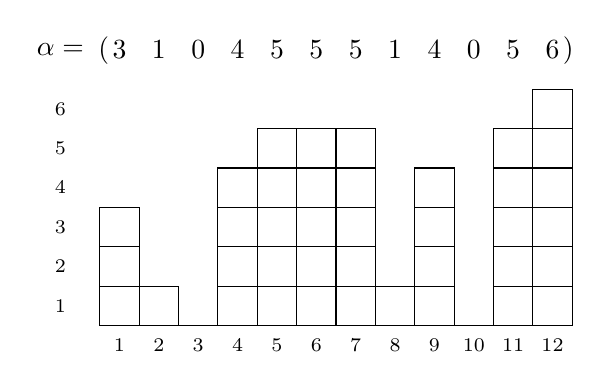
\begin{tikzpicture}[x=.5cm, y=.5cm]
        \node at (0, 8) {\(\alpha = \)};
        \node at (1.1, 7.98) {\((\)};
        \node at (12.9, 7.98) {\()\)};
        \foreach \height [count = \column] in {3, 1, 0, 4, 5, 5, 5, 1, 4, 0, 5, 6}{
          \node at (\column + .5, 8) {\height};
          \foreach \row in {0,...,\height}{
              \ifnum \row = 0
              \else
                \draw[black] (\column, \row) rectangle (\column + 1, \row + 1);
              \fi
            }
          \node at (\column + .5, .5) {\(\scriptstyle \column\)};
          }
        \foreach \row in {1, 2, 3, 4, 5, 6}{
            \node at (0, \row + .5) {\(\scriptstyle \row\)};
          }
        \draw (1,1) -- (13,1);
      \end{tikzpicture}
    \end{center}
\end{frame}

\begin{frame}{Leg, attacking, arm sets of \(u = (i, r)\)}
  \begin{minipage}[t]{.3\textwidth}
    \uncover<1->{
      \begin{center}
        The leg set of \(u\):
      \end{center}
    }
  \end{minipage}
  \hfill
  \begin{minipage}[t]{.3\textwidth}
    % \(\Attack(u) = \{(j, r) : j > i\} \cup \{(j, r - 1) : j < i\}\)
    \uncover<2->{
      \begin{center}
        The attacking set of \(u\):\\[.5em]
        ``\(u\) attacks \(v \in \Attack(u)\)''
      \end{center}
    }
  \end{minipage}
  \hfill
  \begin{minipage}[t]{.3\textwidth}
    \uncover<3->{
      \begin{center}
        The arm set of \(u\):
      \end{center}
    }
  \end{minipage}

  \vspace{2em}

  \begin{center}
    \uncover<1->{
    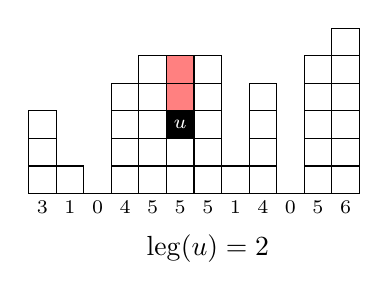
\begin{tikzpicture}[x=.5cm, y=.5cm, scale=.7, baseline={(0,0)}]
      \fill[black] (6,3) rectangle ++(1,1);
      \node[white] at (6.5, 3.5) {\(\scriptstyle u\)};
      \fill[red!50] (6,4) rectangle ++(1,1);
      \fill[red!50] (6,5) rectangle ++(1,1);
      \foreach \height [count = \column] in {3, 1, 0, 4, 5, 5, 5, 1, 4, 0, 5, 6}{
        \foreach \row in {0,...,\height}{
            \ifnum \row = 0
            \else
              \draw[black] (\column, \row) rectangle (\column + 1, \row + 1);
            \fi
          }
        \node at (\column + .5, .5) {\(\scriptstyle \height\)};
        }
      \draw (1,1) -- (13,1);
      \node at (7.5, -1) {\(\leg(u) = 2\)};
    \end{tikzpicture}
    }
    \hspace{3em}
    \uncover<2->{
    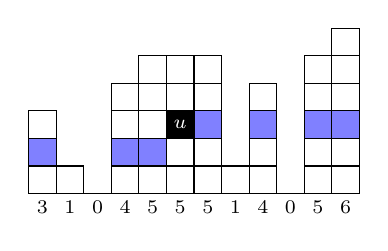
\begin{tikzpicture}[x=.5cm, y=.5cm, scale=.7, baseline={(0,0)}]
      \fill[black] (6,3) rectangle ++(1,1);
      \node[white] at (6.5, 3.5) {\(\scriptstyle u\)};
      \fill[blue!50] (1,2) rectangle ++(1,1);
      \fill[blue!50] (4,2) rectangle ++(1,1);
      \fill[blue!50] (5,2) rectangle ++(1,1);
      \fill[blue!50] (7,3) rectangle ++(1,1);
      \fill[blue!50] (9,3) rectangle ++(1,1);
      \fill[blue!50] (11,3) rectangle ++(1,1);
      \fill[blue!50] (12,3) rectangle ++(1,1);
      \foreach \height [count = \column] in {3, 1, 0, 4, 5, 5, 5, 1, 4, 0, 5, 6}{
        \foreach \row in {0,...,\height}{
            \ifnum \row = 0
            \else
              \draw[black] (\column, \row) rectangle (\column + 1, \row + 1);
            \fi
          }
        \node at (\column + .5, .5) {\(\scriptstyle \height\)};
        }
      \draw (1,1) -- (13,1);
    \end{tikzpicture}
    }
    \hspace{3em}
    \uncover<3->{
    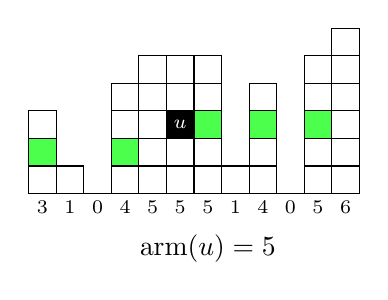
\begin{tikzpicture}[x=.5cm, y=.5cm, scale=.7, baseline={(0,0)}]
      \fill[black] (6,3) rectangle ++(1,1);
      \node[white] at (6.5, 3.5) {\(\scriptstyle u\)};
      \fill[green!70] (1,2) rectangle ++(1,1);
      \fill[green!70] (4,2) rectangle ++(1,1);
      \fill[green!70] (7,3) rectangle ++(1,1);
      \fill[green!70] (9,3) rectangle ++(1,1);
      \fill[green!70] (11,3) rectangle ++(1,1);
      \foreach \height [count = \column] in {3, 1, 0, 4, 5, 5, 5, 1, 4, 0, 5, 6}{
        \foreach \row in {0,...,\height}{
            \ifnum \row = 0
            \else
              \draw[black] (\column, \row) rectangle (\column + 1, \row + 1);
            \fi
          }
        \node at (\column + .5, .5) {\(\scriptstyle \height\)};
        }
      \draw (1,1) -- (13,1);
      \node at (7.5, -1) {\(\arm(u) = 5\)};
    \end{tikzpicture}
    }
  \end{center}
\end{frame}

\begin{frame}{Fillings}
    A \textbf{filling} of shape \(\alpha\) is an assignment of labels (e.g.\,numbers) to the boxes of \(\dg(\alpha)\).

    \begin{center}
      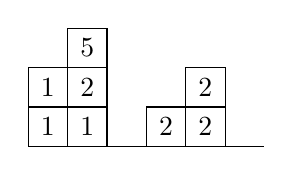
\begin{tikzpicture}[x=.5cm, y=.5cm]
        \def\shape{2, 3, 0, 1, 2, 0}
        \def\filling{
          1, 1,
          1, 2, 5,
          2,
          2, 2}
        \xdef\reading{0}
        \foreach \height [count = \column] in \shape{
          \foreach \row in {0,...,\height}{
              \ifnum \row = 0
              \else
                \pgfmathparse{int(\reading + 1)}
                \xdef\reading{\pgfmathresult}
                \draw[black] (\column, \row) rectangle (\column + 1, \row + 1);
                \coordinate (B\reading) at (\column + .5, \row + .5);
              \fi
            }
        }
        \draw (1,1) -- (7,1);
        \foreach \i [count = \j] in \filling{
          \node at (B\j) {\i};
        }
      \end{tikzpicture}
    \end{center}

  \vspace{2em}

  The \textbf{alphabet} is the set of possible labels in a filling.
  Often (but not always),
  \[\mathcal{A} = [n] = \{1 < 2 < \cdots < n\}\] (the same \(n\) as the number of columns in \(\alpha\), and as the number of variables \(x_1, \dots, x_n\)).
\end{frame}

\begin{frame}{Content of a Filling}
  The \textbf{content} of a filling \(T\) with alphabet \([n]\) is the composition \(\beta = (\beta_1, \beta_2, \dots, \beta_n)\) where
  \[
    \beta_i = \#\{\text{boxes in } T \text{ with label } i\}.
  \]

  \vspace{1em}

  E.g.~ a filling of content
  \((\textcolor<2>{red!80!black}{3},
    \textcolor<3>{red!80!black}{4},
    0,
    0,
    \textcolor<4>{red!80!black}{1},
    0)\):
  \begin{center}
    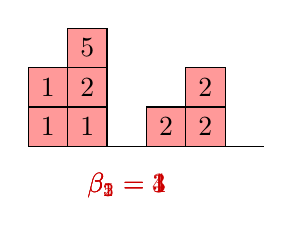
\begin{tikzpicture}[x=.5cm, y=.5cm]
      \def\shape{2, 3, 0, 1, 2, 0}
      \def\filling{
        1, 1,
        1, 2, 5,
        2,
        2, 2}
      \xdef\reading{0}
      \foreach \height [count = \column] in \shape{
        \foreach \row in {0,...,\height}{
            \ifnum \row = 0
            \else
              \pgfmathparse{int(\reading + 1)}
              \xdef\reading{\pgfmathresult}
              \draw[black] (\column, \row) rectangle (\column + 1, \row + 1);
              \coordinate (B\reading) at (\column + .5, \row + .5);
            \fi
          }
      }
      \draw (1,1) -- (7,1);
      \foreach \i [count = \j] in \filling{
        \onslide<2>{
          \ifnum \i = 1
            \draw[fill=red!40] (B\j) ++ (-.5, -.5) rectangle ++(1, 1);
          \fi
        }
        \onslide<3>{
          \ifnum \i = 2
            \draw[fill=red!40] (B\j) ++ (-.5, -.5) rectangle ++(1, 1);
          \fi
        }
        \onslide<4>{
          \ifnum \i = 5
            \draw[fill=red!40] (B\j) ++ (-.5, -.5) rectangle ++(1, 1);
          \fi
        }
        \node at (B\j) {\i};
      }
      \onslide<2>{\node[red!80!black] at (3.5, 0) {\(\beta_1 = 3\)};}
      \onslide<3>{\node[red!80!black] at (3.5, 0) {\(\beta_2 = 4\)};}
      \onslide<4>{\node[red!80!black] at (3.5, 0) {\(\beta_5 = 1\)};}
    \end{tikzpicture}
  \end{center}
  
  \onslide<5->{
  Corresponds to the monomial
  \[
    x^T = x_1^3 x_2^4 x_5^1.
  \]
  }
\end{frame}

\begin{frame}{Statistics of Fillings: \(\maj\) and \(\inv\)/\(\coinv\)}
  \begin{itemize}
    \item major index:
    \uncover<2->{ \(\maj(T) = \displaystyle \sum_{T(u) > T(d(u))} (1 + \leg(u))\),
\begin{figure}[h]
	\begin{tikzpicture}[x=.5cm, y=.5cm, scale=.7]
		\def\shape{2, 2, 0, 1}
		\def\filling{
			3, 1, \textbf2,
			1, \textbf2, \textbf4,
			2,
			4, 4}
    \draw[white] (0,1) rectangle (6,3.5);
		\xdef\reading{0}
        \fill[black!20] (1,2) rectangle ++(1,1);
        \fill[black!20] (2,1) rectangle ++(1,1);
        \fill[black!20] (2,2) rectangle ++(1,1);
        \only<3>{
          \draw[thick, red!80!black] (1.5, 2.5) circle (.8);
        }
        \only<4>{
          \draw[thick, red!80!black] (2.5, 2.5) circle (.8);
        }
        \only<5>{
          \draw[thick, red!80!black] (2.5, 1.5) circle (.8);
        }
		\foreach \height [count = \column] in \shape{
			\foreach \row in {0,...,\height}{
					\pgfmathparse{int(\reading + 1)}
					\xdef\reading{\pgfmathresult}
					\draw[black] (\column, \row) rectangle (\column + 1, \row + 1);
					\coordinate (B\reading) at (\column + .5, \row + .5);
				}
		}
		\foreach \i [count = \j] in \filling{
			\node at (B\j) {\footnotesize \i};
		}
	\end{tikzpicture}
\end{figure}
\[
\maj(T) = \textcolor<3>{red!80!black}{1} + \textcolor<4>{red!80!black}{1} + \textcolor<5>{red!80!black}{2} = 4
\]}

    \item inversion/coinversion number: \onslide<8->{\(\inv(T) = \#\{ \text{inversion triples} \}\), \(\coinv(T) = \#\{ \text{coinversion triples} \}\)}
\end{itemize}

    \onslide<7->{
\begin{center}
	\ytableausetup{smalltableaux}
	\colorlet{inversion}{orange!70!white}
	\colorlet{coinversion}{purple!50!white}
	\renewcommand{\arraystretch}{1.5}
  \scalebox{.85}{
	\begin{tabular}{cccccccccc}
		\begin{ytableau}
			*(coinversion) \textbf2 & *(coinversion) \textbf4 \\
			*(coinversion) \textbf1 & 2 & \none & 4 \\
			3 & 1 & 2 & 4
		\end{ytableau}
		&
		\begin{ytableau}
			2 & 4 \\
			*(coinversion) \textbf1 & *(coinversion) \textbf2 & \none & 4 \\
			*(coinversion) \textbf3 & 1 & 2 & 4
		\end{ytableau}
		&
		\begin{ytableau}
			2 & 4 \\
			*(inversion) \textbf1 & 2 & \none & *(inversion) \textbf4 \\
			*(inversion) \textbf3 & 1 & 2 & 4
		\end{ytableau}
		&
		\begin{ytableau}
			2 & 4 \\
			1 & *(coinversion) \textbf2 & \none & *(coinversion) \textbf4 \\
			3 & *(coinversion) \textbf1 & 2 & 4
		\end{ytableau}
		&
		\begin{ytableau}
			2 & 4 \\
			1 & 2 & \none & *(inversion) \textbf4 \\
			3 & 1 & *(inversion) \textbf2 & *(inversion) \textbf4
		\end{ytableau}
		&
		\begin{ytableau}
			2 & 4 \\
			1 & 2 & \none & 4 \\
			*(inversion) \textbf3 & *(inversion) \textbf1 & 2 & 4
		\end{ytableau}
		&
		\begin{ytableau}
			2 & 4 \\
			1 & 2 & \none & 4 \\
			*(inversion) \textbf3 & 1 & *(inversion) \textbf2 & 4
		\end{ytableau}
		&
		\begin{ytableau}
			2 & 4 \\
			1 & 2 & \none & 4 \\
			*(coinversion) \textbf3 & 1 & 2 & *(coinversion) \textbf4
		\end{ytableau}
		&
		\begin{ytableau}
			2 & 4 \\
			1 & 2 & \none & 4 \\
			3 & *(coinversion) \textbf1 & *(coinversion) \textbf2 & 4
		\end{ytableau}
		&
		\begin{ytableau}
			2 & 4 \\
			1 & 2 & \none & 4 \\
			3 & *(coinversion) \textbf1 & 2 & *(coinversion) \textbf4
		\end{ytableau}
		\\
    \small
		\(1 < 2 < 4\)
		&
    \small
		\(1 < 2 < 3\)
		&
    \small
		\(4 > 3 > 1\)
		&
    \small
		\(1 < 2 < 4\)
		&
    \small
		\(4 \geq 4 > 2\)
    &
    \small
    \(3 > 1\)
    &
    \small
    \(3 > 2\)
    &
    \small
    \(3 < 4\)
    &
    \small
    \(1 < 2\)
    &
    \small
    \(1 < 4\)
	\end{tabular}
  }
\end{center}
    }
    \onslide<8->{ \[ \inv(T) = 4, \quad \coinv(T) = 6\] }
\end{frame}

\begin{frame}{Tableaux Formula for Modified \(\tilde{H}_\lambda\)}

  Let \(\lambda'\) denote the conjugate partition of \(\lambda\) (reflect the skyline diagram across the main diagonal).

  \begin{block}{Theorem \parencite{HHL05}}
    The modified Macdonald polynomial \(\tilde{H}_{\lambda'}(x_1, \dots, x_n; q, t)\) is given by
    \[
      \tilde{H}_{\lambda'}(x_1, \dots, x_n; q, t)
      = \sum_{\substack{T \text{ filling} \\ \text{of shape } \lambda}} 
      x^T
      q^{\inv(T)}
      t^{\maj(T)}
    \]
  \end{block}
  
  \pause

  \begin{block}{Rearrangement Property \parencite{HHL08}}
    For any rearrangement \(\textcolor{red!70!black}{\alpha}\) of the parts of \(\lambda\),
    \[
      C_{\textcolor{red!70!black}{\alpha}}(x_1, \dots, x_n; q, t)
      :=
      \sum_{\substack{T \text{ filling} \\ \text{of shape } \textcolor{red!70!black}{\alpha}}} 
      x^T
      q^{\inv(T)}
      t^{\maj(T)}
      = \tilde{H}_{\lambda'}(x_1, \dots, x_n; q, t).
    \]
  \end{block}
\end{frame}

\begin{frame}{Plethysm and Superization}
  Recall
  \[J_\lambda \quad \xleftrightarrow{\text{ plethystic substitution }} \quad \tilde{H}_{\lambda'}\]

  \vspace{2em}

  Combinatorially,
  plethysm corresponds to \textbf{superization},
  which means using a signed alphabet:
  \begin{equation*}
    \mathcal{A}_{\pm} = [n]_{\pm} = \{1 < \bar{1} < 2 < \bar{2} < \cdots < n < \bar{n}\},
  \end{equation*}
  Everything is the mostly the same, except that
  \begin{align*}
    \text{``}a \not > a\text{''} \qquad \text{but } \text{``}\bar{a} > \bar{a}\text{''}.
  \end{align*}

  \vspace{1em}

  \ytableausetup{boxsize=1.5em}

  E.g.~
  \begin{ytableau}
    2 \\ 2
  \end{ytableau}
  is not a descent, but
  \begin{ytableau}
    \overline{2} \\ \overline{2}
  \end{ytableau}
  is a descent.
\end{frame}

\begin{frame}{Signed Tableaux Formula for Integral Form \(J_\lambda\)}
  Recall that
  \[H_{\lambda'}(X; q, t) = \sum_{\substack{T \text{ filling} \\ \text{of shape } \lambda}} 
  x^T
  q^{\inv(T)}
  t^{\maj(T)},
  \qquad
  \text{and}
  \qquad
  J_\lambda(X; q, t) \xleftrightarrow{\text{plethysm}} H_{\lambda'}.
  \]

  \begin{block}{Theorem \parencite{HHL05}}
    The integral form Macdonald polynomial \(J_{\lambda}(x_1, \dots, x_n; q, t)\) is given by
    \[
      J_{\lambda}(x_1, \dots, x_n; q, t)
      = \sum_{\substack{T \text{ signed filling} \\ \text{of shape } \lambda}}
      x^{|T|}
      q^{\maj(T)}
      t^{\coinv(T)}
      (-t)^{\operatorname{neg}(T)},
    \]
    where \(\operatorname{neg}(T)\) is the number of negative labels in \(T\).
  \end{block}
\end{frame}

\begin{frame}{Unsigned Tableaux Formula for Integral Form \(J_\lambda\)}
  Recall
  \[
    J_{\lambda}(x_1, \dots, x_n; q, t)
    = \sum_{\substack{T \text{ signed filling} \\ \text{of shape } \lambda}}
    x^{|T|}
    q^{\maj(T)}
    t^{\coinv(T)}
    (-t)^{\operatorname{neg}(T)},
  \]

  \vspace{1em}

  A filling \(T\) is \textbf{nonattacking} if \(\left|T(u)\right| \neq \left|T(v)\right|\) whenever \(v \in \Attack(u)\).

  \vspace{1em}

  \begin{block}{Theorem \parencite{HHL05}}
    The integral form Macdonald polynomial \(J_{\lambda}(x_1, \dots, x_n; q, t)\) is given by
    \[
      \sum_{\substack{T \text{ nonattacking filling} \\ \text{of shape } \lambda}}
      \mkern-18mu
      x^{T}
      q^{\maj(T)}
      t^{\coinv(T)}
      \prod_{\substack{u \in \dg(\lambda) \\ T(u) = T(\south{u})}}
      (1 - q^{\leg(u) + 1} t^{\arm(u) + 1})
      \prod_{\substack{u \in \dg(\lambda) \\ T(u) \neq T(\south{u}) \\ \text{or } u \text{ in row } 1}}
      (1 - t).
    \]
  \end{block}
\end{frame}

\begin{frame}{Augmented Skyline Diagrams}
    \textbf{\uncover<2->{Augmented} skyline diagram} \(\adg(\alpha)\) of a composition \(\alpha\): \hfill \uncover<2->{(basement = row \(0\) = red)}
    \begin{center}
      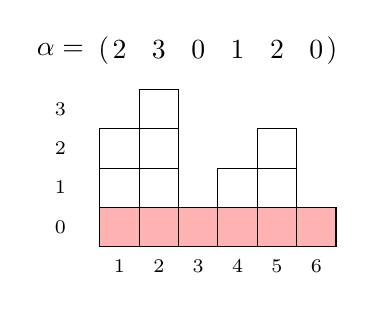
\begin{tikzpicture}[x=.5cm, y=.5cm]
        \node at (0, 5) {\(\alpha = \)};
        \node at (1.1, 4.98) {\((\)};
        \node at (6.9, 4.98) {\()\)};
        \foreach \height [count = \column] in {2, 3, 0, 1, 2, 0}{
          \node at (\column + .5, 5) {\height};
          \foreach \row in {0,...,\height}{
              \ifnum \row = 0
                \uncover<2->{\draw[black,fill=red!30] (\column, \row) rectangle (\column + 1, \row + 1);}
              \else
                \draw[black] (\column, \row) rectangle (\column + 1, \row + 1);
              \fi
            }
          \node at (\column + .5, -.5) {\(\scriptstyle \column\)};
          }
        \foreach \row in {0, 1, 2, 3}{
            \node at (0, \row + .5) {\(\scriptstyle \row\)};
          }
      \end{tikzpicture}
    \end{center}

    \uncover<3->{

    An \textbf{(augmented) filling} \(T\) of shape \(\alpha\) with \textbf{basement} \(\sigma = \window{\sigma_1, \sigma_2, \dots, \sigma_n} \in S_n\) is an assignment \(T \colon \adg(\alpha) \to [n]\) such that \(T(0, i) = \sigma_i\).

    \vspace{1em}

    Signed augmented fillings map to \([n]_{\pm}\), but basement only uses positive (distinct) labels.

    \vspace{.5em}

    \begin{block}{}
      Everything mostly* works the same as before, but with a ``fixed'' row \(0\).\\
      {\footnotesize *Contributions to statistics that only involve basement boxes are ignored.}
    \end{block}
    }
\end{frame}

\begin{frame}{Tableaux Formula for permuted basement \(E_\alpha^\sigma\) and its integral form \(\mathcal{E}_\alpha^\sigma\)}
  \begin{block}{Definition/Theorem \parencite{Fer11}}
    The permuted-basement Macdonald polynomial \(E_\alpha^\sigma(x_1, \dots, x_n; q, t)\) is given by
    \[
      E_\alpha^\sigma
      =
      \sum_{\substack{T \text{ nonattacking filling} \\ \text{of shape } \alpha \\ \text{with basement } \sigma}}
      \mkern-18mu
      x^{T}
      q^{\maj(T)}
      t^{\coinv(T)}
      \prod_{\substack{u \in \dg(\alpha) \\ T(u) \neq T(\south{u})}}
      \frac{1 - t}{1 - q^{\leg(u) + 1} t^{\arm(u) + 1}}.
    \]
  \end{block}

  \begin{block}{Corollary}
    The integral form permuted-basement Macdonald polynomial \(\mathcal{E}_\alpha^\sigma(x_1, \dots, x_n; q, t)\) is given by
    \[
      \mathcal{E}_\alpha^\sigma = 
      \sum_{\substack{T \text{ nonattacking filling} \\ \text{of shape } \alpha \\ \text{with basement } \sigma}}
      \mkern-18mu
      x^{T}
      q^{\maj(T)}
      t^{\coinv(T)}
      \prod_{\substack{u \in \dg(\alpha) \\ T(u) = T(\south{u})}}
      (1 - q^{\leg(u) + 1} t^{\arm(u) + 1})
      \prod_{\substack{u \in \dg(\alpha) \\ T(u) \neq T(\south{u})}}
      (1 - t).
    \]
  \end{block}
\end{frame}

\begin{frame}{Signed Tableaux Formula for permuted basement \(\mathcal{E}_\alpha^\sigma\)}

  The nonattaking formula for \(\mathcal{E}_\alpha^\sigma\) looks similar tot eh nonattacking formula for \(J_\lambda\).

  \vspace{1em}

  Manipulating in the same way as before (but in reverse order) gives:

  \begin{block}{Proposition}
    The integral form permuted-basement Macdonald polynomial \(\mathcal{E}_\alpha^\sigma(x_1, \dots, x_n; q, t)\) is given by
    \[
      \mathcal{E}_\alpha^\sigma(x_1, \dots, x_n; q, t)
      =
      \sum_{\substack{T \text{ signed filling} \\ \text{of shape } \alpha \\ \text{with basement } \sigma}}
      \mkern-18mu
      x^{|T|}
      q^{\maj(T)}
      t^{\coinv(T)}
      (-t)^{\operatorname{neg}(T)}
    \]
  \end{block}
  
  \vspace{1em}
  \pause

  \textit{Aside:} Plethysm doesn't easily generalize from symmetric polynomials to nonsymmetric polynomials. But very recent work by Blasiak--Haiman--Morse--Pun--Seelinger (June 2025 on arXiv) constructs a nonsymmetric plethysm operator.
  
\end{frame}

\part{Breathe, Drink Water, and \\ what have we done with fillings?}

\begin{frame}{Main Results}

    \textbf{Using (deterministic) bijections:}
    \begin{itemize}
        \item 
        For any rearrangement \(\alpha\) of \(\lambda\), we have:
        \[ \tilde{H}_{\lambda'} = C_{\alpha} \qquad \text{from } C_{\alpha} = C_{s_i \alpha}. \]

        \item
        When \(\alpha_i > \alpha_{i+1}\), we have:
        \[
            E_\alpha^\sigma = 
            E_{s_i \alpha}^{\sigma s_i} +
            (\text{coefficient}) \cdot
            E_{s_i \alpha}^\sigma.
        \]
    \end{itemize}

    \textbf{Using probabilistic bijections:}
    \begin{itemize}
        \item
        When \(\alpha_i = \alpha_{i+1}\), we have:
        \[
            E_\alpha^\sigma = E_\alpha^{\sigma s_i}.
        \]
    \end{itemize}
\end{frame}

\part{(Deterministic) Bijections}

\begin{frame}{Goal: Prove \(C_\alpha = C_{s_i \alpha}\)}
  \begin{block}{Goal}
    \[
      \sum_{\substack{T \text{ fillings} \\ \text{of shape } \alpha}}
      x^T q^{\inv(T)} t^{\maj(T)}
      =
      \sum_{\substack{T \text{ fillings} \\ \text{of shape } s_i \alpha}}
      x^T q^{\inv(T)} t^{\maj(T)}
    \]
  \end{block}

  \begin{block}{Combinatorial Goal}
    Construct a bijection between the set of fillings of shape \(\alpha\)
    and the set of fillings of shape \(s_i \alpha\) that preserves content, \(\inv\), and \(\maj\).
  \end{block}
\end{frame}

\begin{frame}{Some structure on this bijeciton}
  \[
    % \{\text{fillings of shape } \composition{\alpha_1, \dots, \alpha_{i-1}, \alpha_i, \alpha_{i+1}, \alpha_{i+2}, \dots, \alpha_n} \}
    % \xrightarrow{\text{bijection}}
    % \{\text{fillings of shape } \composition{\alpha_1, \dots, \alpha_{i-1}, \alpha_{i+1}, \alpha_i, \alpha_{i+2}, \dots, \alpha_n} \}
    \left\{ \begin{array}{c} \text{fillings of shape} \\ \composition{\alpha_1, \dots, \alpha_{i-1}, \alpha_i, \alpha_{i+1}, \alpha_{i+2}, \dots, \alpha_n} \end{array} \right\}
    \xrightarrow{\text{bijection } \phi }
    \left\{ \begin{array}{c} \text{fillings of shape} \\ \composition{\alpha_1, \dots, \alpha_{i-1}, \alpha_{i+1}, \alpha_i, \alpha_{i+2}, \dots, \alpha_n} \end{array} \right\}
  \]

  Without loss of generality, assume \(\alpha_i > \alpha_{i+1}\).

  \begin{itemize}
    \item Columns other than \(i\) and \(i+1\) are unchanged.
    \item The top \(\alpha_i - \alpha_{i+1}\) boxes of column \(i\) are moved to the top of column \(i+1\).
    \item Each row \(r \in \{1, 2, \dots, \alpha_{i+1}\}\) are either \textbf{copied as is}, or are \textbf{swapped} between columns \(i\) and \(i+1\).
  \end{itemize}

  \begin{center}
    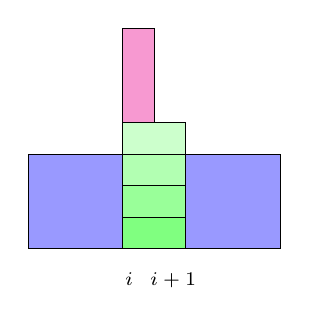
\begin{tikzpicture}[scale=.4]
      \draw[fill = blue!40] (0, 0) rectangle (3, 3);
      \draw[fill = magenta!40] (3, 4) rectangle (4, 7);
      \draw[fill = blue!40] (5, 0) rectangle (8, 3);
      \draw[fill = green!50] (3, 0) rectangle (5, 1);
      \draw[fill = green!40] (3, 1) rectangle (5, 2);
      \draw[fill = green!30] (3, 2) rectangle (5, 3);
      \draw[fill = green!20] (3, 3) rectangle (5, 4);
      \node at (3.2, -.95) {\scriptsize \(i\)};
      \node at (4.6, -1) {\scriptsize \({i+1}\)};
    \end{tikzpicture}
    \raisebox{3em}{\(\xrightarrow{\phi}\)}
    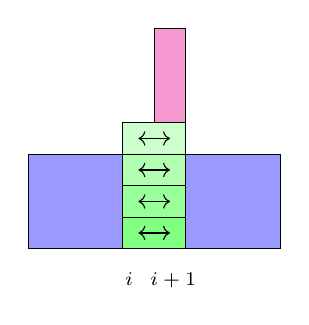
\begin{tikzpicture}[scale=.4]
      \draw[fill = blue!40] (0, 0) rectangle (3, 3);
      \draw[fill = magenta!40] (4, 4) rectangle (5, 7);
      \draw[fill = blue!40] (5, 0) rectangle (8, 3);
      \draw[fill = green!50] (3, 0) rectangle (5, 1);
      \draw[fill = green!40] (3, 1) rectangle (5, 2);
      \draw[fill = green!30] (3, 2) rectangle (5, 3);
      \draw[fill = green!20] (3, 3) rectangle (5, 4);
      \node at (3.2, -.95) {\scriptsize \(i\)};
      \node at (4.6, -1) {\scriptsize \({i+1}\)};
      \draw[<->] (3.5, 0.5) -- (4.5, 0.5);
      \draw[<->] (3.5, 1.5) -- (4.5, 1.5);
      \draw[<->] (3.5, 2.5) -- (4.5, 2.5);
      \draw[<->] (3.5, 3.5) -- (4.5, 3.5);
    \end{tikzpicture}
  \end{center}
\end{frame}

\begin{frame}{Idea: Split into blocks}
  \begin{minipage}{0.4\textwidth}
    \centering
      \begin{ytableau}
        \none[{\scriptstyle \text{row }r+1}] & \none & a & b \\
        \none[{\scriptstyle \text{row }r}] & \none & c & d 
      \end{ytableau}\\[1em]
      \textbf{not intertwined:}\\[1em]
        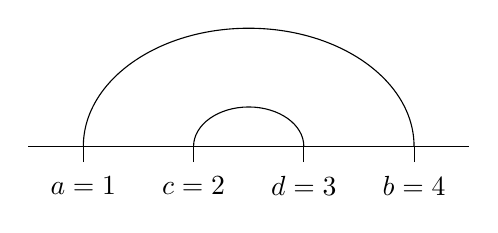
\begin{tikzpicture}[x=1.4cm]
            \node at (0, 0.5) {\(a = 1\)};
            \node at (1, 0.5) {\(c = 2\)};
            \node at (2, 0.5) {\(d = 3\)};
            \node at (3, 0.5) {\(b = 4\)};
            \draw (-.5, 1) -- (3.5, 1);
            \draw (0, .8) -- (0, 1);
            \draw (1, .8) -- (1, 1);
            \draw (2, .8) -- (2, 1);
            \draw (3, .8) -- (3, 1);
            \draw (0, 1) arc (180:0:1.5);
            \draw (1, 1) arc (180:0:0.5);
        \end{tikzpicture}\\[2em]
      \textbf{intertwined:}\\[1em]
        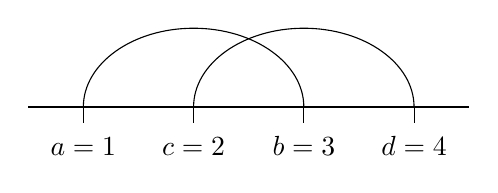
\begin{tikzpicture}[x=1.4cm]
            \node at (0, 0.5) {\(a = 1\)};
            \node at (1, 0.5) {\(c = 2\)};
            \node at (2, 0.5) {\(b = 3\)};
            \node at (3, 0.5) {\(d = 4\)};
            \draw (-.5, 1) -- (3.5, 1);
            \draw (0, .8) -- (0, 1);
            \draw (1, .8) -- (1, 1);
            \draw (2, .8) -- (2, 1);
            \draw (3, .8) -- (3, 1);
            \draw (0, 1) arc (180:0:1);
            \draw (1, 1) arc (180:0:1);
        \end{tikzpicture}
  \end{minipage} \hfill
  \begin{minipage}{0.55\textwidth}
    \pause
    \begin{center}
      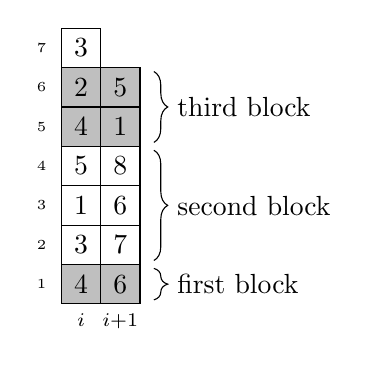
\begin{tikzpicture}[scale=.5]
        \node at (-0.5, 7.5) {\tiny \(7\)};
        \node at (-0.5, 6.5) {\tiny \(6\)};
        \node at (-0.5, 5.5) {\tiny \(5\)};
        \node at (-0.5, 4.5) {\tiny \(4\)};
        \node at (-0.5, 3.5) {\tiny \(3\)};
        \node at (-0.5, 2.5) {\tiny \(2\)};
        \node at (-0.5, 1.5) {\tiny \(1\)};
        \node[anchor=north] at (0.5, 1) {\(\scriptstyle i\)};
        \node[anchor=north] at (1.5, 1) {\(\scriptstyle i+1\)};
        \draw (0, 7) rectangle ++(1, 1);
        \draw (1, 6) rectangle ++(1, 1)[fill=gray!50];
        \draw (0, 6) rectangle ++(1, 1)[fill=gray!50];
        \draw (1, 5) rectangle ++(1, 1)[fill=gray!50];
        \draw (0, 5) rectangle ++(1, 1)[fill=gray!50];
        \draw (1, 4) rectangle ++(1, 1);
        \draw (0, 4) rectangle ++(1, 1);
        \draw (1, 3) rectangle ++(1, 1);
        \draw (0, 3) rectangle ++(1, 1);
        \draw (1, 2) rectangle ++(1, 1);
        \draw (0, 2) rectangle ++(1, 1);
        \draw (1, 1) rectangle ++(1, 1)[fill=gray!50];
        \draw (0, 1) rectangle ++(1, 1)[fill=gray!50];
        \node at (0.5, 7.5) {\(3\)};
        \node at (1.5, 6.5) {\(5\)};
        \node at (0.5, 6.5) {\(2\)};
        \node at (1.5, 5.5) {\(1\)};
        \node at (0.5, 5.5) {\(4\)};
        \node at (1.5, 4.5) {\(8\)};
        \node at (0.5, 4.5) {\(5\)};
        \node at (1.5, 3.5) {\(6\)};
        \node at (0.5, 3.5) {\(1\)};
        \node at (1.5, 2.5) {\(7\)};
        \node at (0.5, 2.5) {\(3\)};
        \node at (1.5, 1.5) {\(6\)};
        \node at (0.5, 1.5) {\(4\)};
        \draw[decorate, decoration={brace, amplitude=5pt, mirror, raise=5pt}] (2, 5.1) -- (2, 6.9) node[midway, anchor=west, xshift=10pt] {third block};
        \draw[decorate, decoration={brace, amplitude=5pt, mirror, raise=5pt}] (2, 2.1) -- (2, 4.9) node[midway, anchor=west, xshift=10pt] {second block};
        \draw[decorate, decoration={brace, amplitude=5pt, mirror, raise=5pt}] (2, 1.1) -- (2, 1.9) node[midway, anchor=west, xshift=10pt] {first block};
      \end{tikzpicture}
    \end{center}
      
    \vspace{1em}

    \pause

    The map \(\phi\) copy the blocks as is, or swaps all rows in the block.

    \vspace{.5em}

    This requirement takes care of the inversion triples inside each block.
  \end{minipage}
\end{frame}

\begin{frame}{To swap or not to swap (each block)?}
  \begin{minipage}[c]{.3\textwidth}
    \centering
	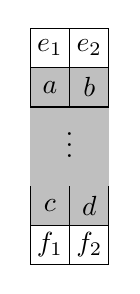
\begin{tikzpicture}[scale=.5]
		\draw (0, 0) rectangle ++(1, 1);
		\draw (1, 0) rectangle ++(1, 1);
		\draw[fill=gray!50] (0, 1) rectangle ++(1, 1);
		\draw[fill=gray!50] (1, 1) rectangle ++(1, 1);
		\fill[gray!50] (0, 2) rectangle ++(2, 2);
		\node at (1, 3.25) {\(\vdots\)};
		\draw[fill=gray!50] (0, 4) rectangle ++(1, 1);
		\draw[fill=gray!50] (1, 4) rectangle ++(1, 1);
		\draw (0, 5) rectangle ++(1, 1);
		\draw (1, 5) rectangle ++(1, 1);
		\node at (0.5, 5.5) {\(e_1\)};
		\node at (1.5, 5.5) {\(e_2\)};
		\node at (0.5, 4.5) {\(a\)};
		\node at (1.5, 4.5) {\(b\)};
		\node at (0.5, 1.5) {\(c\)};
		\node at (1.5, 1.5) {\(d\)};
		\node at (0.5, 0.5) {\(f_1\)};
		\node at (1.5, 0.5) {\(f_2\)};
	\end{tikzpicture}
  \end{minipage}
  \begin{minipage}[c]{0.65\textwidth}
    \pause
    Swap the block if and only if the triples
    \[
      \begin{ytableau}
        \none & e_\bullet \\
        a & b
      \end{ytableau}
      \text{ and }
      \begin{ytableau}
        c & d \\
        f_\bullet & \none
      \end{ytableau}
    \]
    have different inversion type.

    \vspace{1em}

    \pause

    \begin{block}{Theorem}
      The map \(\phi\) is a bijection that preserves content, \(\inv\), and \(\maj\)!
    \end{block}

    \begin{block}{Corollary}
      For any rearrangement \(\alpha\) of \(\lambda\),
      \[ H_{\lambda'} = \textstyle \sum_{\substack{T \text{ filling of shape } \alpha}} 
      x^T
      q^{\inv(T)}
      t^{\maj(T)}.
      \]
    \end{block}
  \end{minipage}
\end{frame}

\begin{frame}{Example of \(\phi\)}
  \centering

    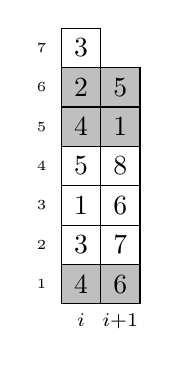
\begin{tikzpicture}[scale=.5]
      \node at (-0.5, 7.5) {\tiny \(7\)};
      \node at (-0.5, 6.5) {\tiny \(6\)};
      \node at (-0.5, 5.5) {\tiny \(5\)};
      \node at (-0.5, 4.5) {\tiny \(4\)};
      \node at (-0.5, 3.5) {\tiny \(3\)};
      \node at (-0.5, 2.5) {\tiny \(2\)};
      \node at (-0.5, 1.5) {\tiny \(1\)};
      \node[anchor=north] at (0.5, 1) {\(\scriptstyle i\)};
      \node[anchor=north] at (1.5, 1) {\(\scriptstyle i+1\)};
      \draw (0, 7) rectangle ++(1, 1);
      \draw (1, 6) rectangle ++(1, 1)[fill=gray!50];
      \draw (0, 6) rectangle ++(1, 1)[fill=gray!50];
      \draw (1, 5) rectangle ++(1, 1)[fill=gray!50];
      \draw (0, 5) rectangle ++(1, 1)[fill=gray!50];
      \draw (1, 4) rectangle ++(1, 1);
      \draw (0, 4) rectangle ++(1, 1);
      \draw (1, 3) rectangle ++(1, 1);
      \draw (0, 3) rectangle ++(1, 1);
      \draw (1, 2) rectangle ++(1, 1);
      \draw (0, 2) rectangle ++(1, 1);
      \draw (1, 1) rectangle ++(1, 1)[fill=gray!50];
      \draw (0, 1) rectangle ++(1, 1)[fill=gray!50];
      \node at (0.5, 7.5) {\(3\)};
      \node at (1.5, 6.5) {\(5\)};
      \node at (0.5, 6.5) {\(2\)};
      \node at (1.5, 5.5) {\(1\)};
      \node at (0.5, 5.5) {\(4\)};
      \node at (1.5, 4.5) {\(8\)};
      \node at (0.5, 4.5) {\(5\)};
      \node at (1.5, 3.5) {\(6\)};
      \node at (0.5, 3.5) {\(1\)};
      \node at (1.5, 2.5) {\(7\)};
      \node at (0.5, 2.5) {\(3\)};
      \node at (1.5, 1.5) {\(6\)};
      \node at (0.5, 1.5) {\(4\)};
    \end{tikzpicture}
    \qquad \raisebox{2cm}{\(\xrightarrow{\phi}\)} \qquad
	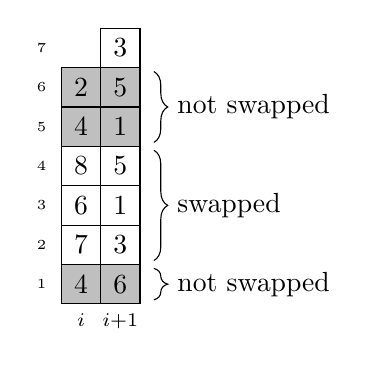
\begin{tikzpicture}[scale=.5]
		\node at (-0.5, 7.5) {\tiny \(7\)};
		\node at (-0.5, 6.5) {\tiny \(6\)};
		\node at (-0.5, 5.5) {\tiny \(5\)};
		\node at (-0.5, 4.5) {\tiny \(4\)};
		\node at (-0.5, 3.5) {\tiny \(3\)};
		\node at (-0.5, 2.5) {\tiny \(2\)};
		\node at (-0.5, 1.5) {\tiny \(1\)};
		\node[anchor=north] at (0.5, 1) {\(\scriptstyle i\)};
		\node[anchor=north] at (1.5, 1) {\(\scriptstyle i+1\)};
		\draw (1, 7) rectangle ++(1, 1);
		\draw (1, 6) rectangle ++(1, 1)[fill=gray!50];
		\draw (0, 6) rectangle ++(1, 1)[fill=gray!50];
		\draw (1, 5) rectangle ++(1, 1)[fill=gray!50];
		\draw (0, 5) rectangle ++(1, 1)[fill=gray!50];
		\draw (1, 4) rectangle ++(1, 1);
		\draw (0, 4) rectangle ++(1, 1);
		\draw (1, 3) rectangle ++(1, 1);
		\draw (0, 3) rectangle ++(1, 1);
		\draw (1, 2) rectangle ++(1, 1);
		\draw (0, 2) rectangle ++(1, 1);
		\draw (1, 1) rectangle ++(1, 1)[fill=gray!50];
		\draw (0, 1) rectangle ++(1, 1)[fill=gray!50];
		\node at (1.5, 7.5) {\(3\)};
		\node at (1.5, 6.5) {\(5\)};
		\node at (0.5, 6.5) {\(2\)};
		\node at (1.5, 5.5) {\(1\)};
		\node at (0.5, 5.5) {\(4\)};
		\node at (1.5, 4.5) {\(5\)};
		\node at (0.5, 4.5) {\(8\)};
		\node at (1.5, 3.5) {\(1\)};
		\node at (0.5, 3.5) {\(6\)};
		\node at (1.5, 2.5) {\(3\)};
		\node at (0.5, 2.5) {\(7\)};
		\node at (1.5, 1.5) {\(6\)};
		\node at (0.5, 1.5) {\(4\)};
		\draw[decorate, decoration={brace, amplitude=5pt, mirror, raise=5pt}] (2, 5.1) -- (2, 6.9) node[midway, anchor=west, xshift=10pt] {not swapped};
		\draw[decorate, decoration={brace, amplitude=5pt, mirror, raise=5pt}] (2, 2.1) -- (2, 4.9) node[midway, anchor=west, xshift=10pt] {swapped};
		\draw[decorate, decoration={brace, amplitude=5pt, mirror, raise=5pt}] (2, 1.1) -- (2, 1.9) node[midway, anchor=west, xshift=10pt] {not swapped};
	\end{tikzpicture}
\end{frame}

\begin{frame}{Second goal with bijections}
  \begin{block}{Goal}
    When \(\alpha_i > \alpha_{i+1}\), prove
    \(
      E_\alpha^\sigma = 
      E_{s_i \alpha}^{\sigma s_i} +
      (\text{coefficient}) \cdot
      E_{s_i \alpha}^\sigma,
    \)
    that is,
    \[
      \textstyle
      \sum_{\substack{T \text{ signed fillings} \\ \text{of shape } \alpha \\ \text{with basement } \sigma}}
      \wt(T)
      =
      \sum_{\substack{U \text{ signed fillings} \\ \text{of shape } s_i \alpha \\ \text{with basement } \sigma s_i}}
      \wt(U)
      +
      (\text{coefficient}) \cdot
      \sum_{\substack{V \text{ signed fillings} \\ \text{of shape } s_i \alpha \\ \text{with basement } \sigma}}
      \wt(V).
    \]
  \end{block}

  \begin{block}{Combinatorial Goal}
    Construct bijections
    \begin{gather*}
      f \colon \left\{ \begin{array}{c} \text{signed fillings of shape} \\ \alpha \text{ with basement } \sigma \end{array} \right\}
      \to
      \left\{ \begin{array}{c} \text{signed fillings of shape} \\ s_i \alpha \text{ with basement } \sigma s_i \end{array} \right\} \\
      g \colon \left\{ \begin{array}{c} \text{signed fillings of shape} \\ \alpha \text{ with basement } \sigma \end{array} \right\}
      \to
      \left\{ \begin{array}{c} \text{signed fillings of shape} \\ s_i \alpha \text{ with basement } \sigma \end{array} \right\}
    \end{gather*}
    such that, for all \(T\),
    \[
    \wt(T) = \wt(f(T)) + (\text{coefficient}) \cdot \wt(g(T)).
    \]
  \end{block}
\end{frame}

\begin{frame}{The new bijections \(f\) and \(g\)}
  Naively applying the previous bijection \(\phi\) \textbf{might or might not} swap \(\sigma_i\) and \(\sigma_{i+1}\) in the basement.
  \[
    \phi \colon \operatorname{Fill}_\pm(\alpha, \sigma)
    \to
    \operatorname{Fill}_\pm(s_i \alpha, \sigma s_i)
    \cup
    \operatorname{Fill}_\pm(s_i \alpha, \sigma).
  \]

  Define \(\psi\) to be the same as \(\phi\), except do the opposite action on the bottom block.
  \[
    \psi \colon \operatorname{Fill}_\pm(\alpha, \sigma)
    \to
    \operatorname{Fill}_\pm(s_i \alpha, \sigma)
    \cup
    \operatorname{Fill}_\pm(s_i \alpha, \sigma s_i).
  \]

  \begin{block}{Proposition}
    The map \(\psi\) changes \(\inv\) and \(\maj\) in a predictable way. 
    (That's where the coefficient comes from.)
  \end{block}

  \vspace{.5em}

  Define \(f\) and \(g\) such that
  \[
    \{f(T), g(T)\} = \{\phi(T), \psi(T)\}
  \]
  in the correct order so that \(f(T)\) has basement \(\sigma s_i\) and \(g(T)\) has basement \(\sigma\).
\end{frame}

\begin{frame}{The bijections \(f\) and \(g\) work!}
  Define \(f\) and \(g\) such that
  \[
    \{f(T), g(T)\} = \{\phi(T), \psi(T)\}
  \]
  in the correct order so that \(f(T)\) has basement \(\sigma s_i\) and \(g(T)\) has basement \(\sigma\).

  \begin{block}{Lemma}
    The maps \(f\) and \(g\) are bijections such that, for all \(T\),
    \[
    \wt(T) = \wt(f(T)) + (\text{coefficient}) \cdot \wt(g(T)).
    \]
  \end{block}

  \begin{block}{Corollary}
    When \(\alpha_i > \alpha_{i+1}\), we have:
    \[
      E_\alpha^\sigma = 
      E_{s_i \alpha}^{\sigma s_i} +
      (\text{coefficient}) \cdot
      E_{s_i \alpha}^\sigma.
    \]
  \end{block}
\end{frame}

\part{Probabilistic Bijections}

\begin{frame}{Generalizing the goal: $F = G$}
  $F$ and $G$ are weight generating functions of $\textbf{S}$ and $\textbf{T}$.
  How to combinatorially prove \[ F = G \ ? \]

  \pause

  \begin{block}{A strategy}
    Construct a \textbf{weight-preserving bijection} between $\textbf{S}$ and $\textbf{T}$.
  \end{block}
\end{frame}

\begin{frame}{Weight-preserving Bijections}
  \textbf{Weight-preserving bijections:}
  \[
    f \colon \textbf{S} \to \textbf{T} \qquad \text{with an inverse} \qquad g \colon \textbf{T} \to \textbf{S}
  \]
  such that, whenever $f(S) = T$, we have
  \[ \operatorname{wt}(S) = \operatorname{wt}(T). \]

  \vspace{-.75em}
  \pause

  \begin{prop}
    If there exists a weight-preserving bijection between \(\mathbf{S}\) and \(\mathbf{T}\), then
    \[ \sum_{S \in \mathbf{S}} \operatorname{wt}(S) = \sum_{T \in \mathbf{T}} \operatorname{wt}(T). \]
  \end{prop}

  \pause

  \begin{center}
  \textbf{What about when it's hard (or impossible) to find a weight-preserving bijection?}
  \end{center}
\end{frame}

\begin{frame}{Probabilistic Bijections}
  \setlength{\abovedisplayskip}{2pt}
  \setlength{\belowdisplayskip}{2pt}
  \setlength{\abovedisplayshortskip}{2pt}
  \setlength{\belowdisplayshortskip}{2pt}
  \textbf{Probabilistic bijection:} pair of maps to an algebra \(A\) \hfill {\small \parencite{FS24}}
  \begin{equation*}
    \operatorname{prob}_{\mathbf{S}} \colon \mathbf{S} \times \mathbf{T} \to A
    \quad \text{and} \quad
    \operatorname{prob}_{\mathbf{T}} \colon \mathbf{T} \times \mathbf{S} \to A
  \end{equation*}
  such that, for all \(S \in \mathbf{S}\) and \(T \in \mathbf{T}\),
  \vspace{1em}
  \pause
  \begin{itemize}
    \item \textbf{probabilities sum to 1:}
    $ \displaystyle \sum_{T \in \mathbf{T}} \operatorname{prob}_{\mathbf{S}}(S, T) = 1 $
    and
    $ \displaystyle \sum_{S \in \mathbf{S}} \operatorname{prob}_{\mathbf{T}}(T, S) = 1 $,
    \pause
    \vspace{1em}
    \item \textbf{balance condition:}
    $ \operatorname{wt}(S) \operatorname{prob}_{\mathbf{S}}(S, T) = \operatorname{wt}(T) \operatorname{prob}_{\mathbf{T}}(T, S) $.
  \end{itemize}
  \pause
  \begin{prop}
    If there exists a probabilistic bijection between \(\mathbf{S}\) and \(\mathbf{T}\), then
    \[ \sum_{S \in \mathbf{S}} \operatorname{wt}(S) = \sum_{T \in \mathbf{T}} \operatorname{wt}(T). \]
  \end{prop}
\end{frame}

\begin{frame}{Proof of Proposition}
  \begin{prop}
    If there exists a probabilistic bijection between \(\mathbf{S}\) and \(\mathbf{T}\), then
    \[ \sum_{S \in \mathbf{S}} \operatorname{wt}(S) = \sum_{T \in \mathbf{T}} \operatorname{wt}(T). \]
  \end{prop}

  \begin{block}{Proof}
    \vspace{-1em}
    \begin{align*}
      \sum_{S \in \mathbf{S}} 1 \cdot \operatorname{wt}(S)
       & \uncover<+(1)->{ = \sum_{S \in \mathbf{S}} \sum_{T \in \mathbf{T}} \operatorname{prob}_{\mathbf{S}}(S, T) \operatorname{wt}(S) & \text{(probabilities sum to \(1\))} } \\
       & \uncover<+(1)->{ = \sum_{T \in \mathbf{T}} \sum_{S \in \mathbf{S}} \operatorname{prob}_{\mathbf{T}}(T, S) \operatorname{wt}(T) & \text{(balance condition)} } \\
       & \uncover<+(1)->{ = \sum_{T \in \mathbf{T}} 1 \cdot \operatorname{wt}(T). & \text{(probabilities sum to \(1\))} }
    \end{align*}

    \vspace{-1.5em}

    \  \hfill \(\square\)
  \end{block}
\end{frame}

\begin{frame}{Example (Spoiler)}
  \centering
  \ytableausetup{smalltableaux, centertableaux}
  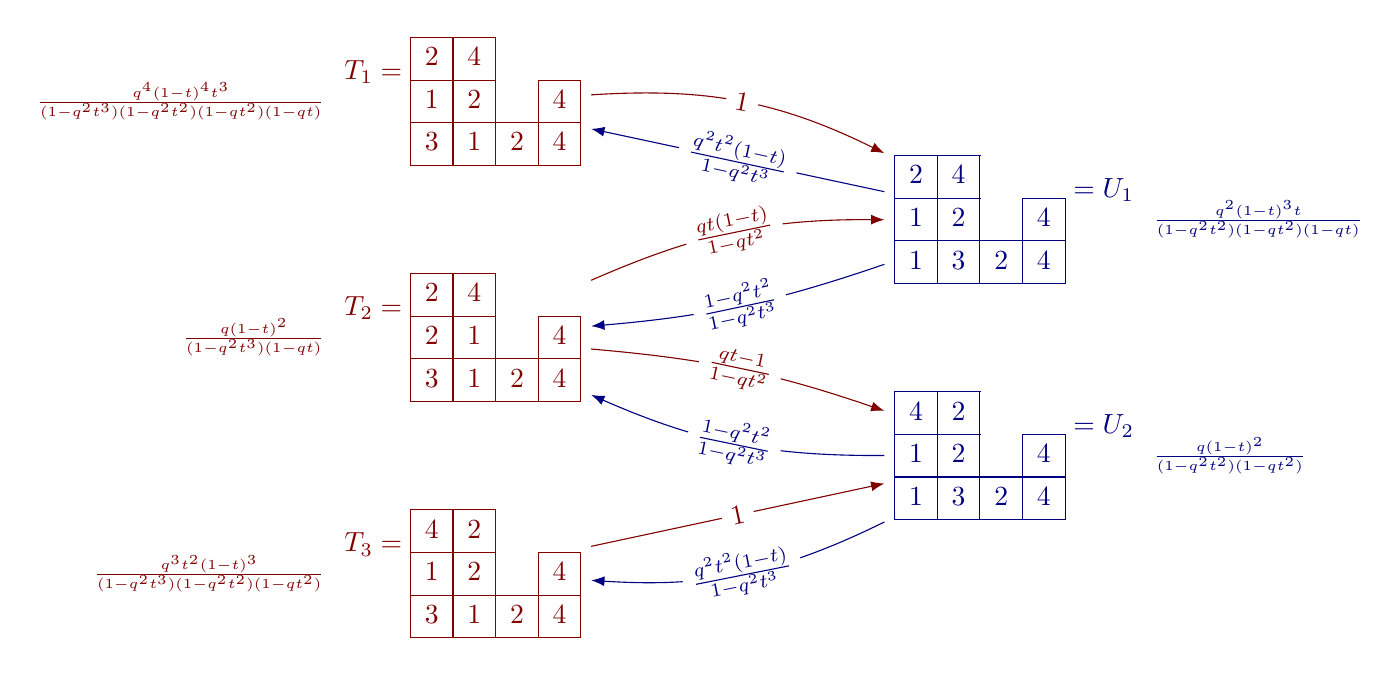
\begin{tikzpicture}
    \node[red!50!black]  (T1) at (-4,  3) {
      $T_1 =
        \begin{ytableau}
          2 & 4 \\
          1 & 2 & \none & 4 \\
          3 & 1 & 2 & 4
        \end{ytableau}$
    };
    \node[red!50!black]  (T2) at (-4,  0) {
      $T_2 =
        \begin{ytableau}
          2 & 4 \\
          2 & 1 & \none & 4 \\
          3 & 1 & 2 & 4
        \end{ytableau}$
    };
    \node[red!50!black]  (T3) at (-4, -3) {
      $T_3 =
        \begin{ytableau}
          4 & 2 \\
          1 & 2 & \none & 4 \\
          3 & 1 & 2 & 4
        \end{ytableau}$
    };
    \node[blue!50!black] (U1) at ( 3,  1.5) {
      $\begin{ytableau}
          2 & 4 \\
          1 & 2 & \none & 4 \\
          1 & 3 & 2 & 4
        \end{ytableau} = U_1$
    };
    \node[blue!50!black] (U2) at ( 3, -1.5) {
      $\begin{ytableau}
          4 & 2 \\
          1 & 2 & \none & 4 \\
          1 & 3 & 2 & 4
        \end{ytableau} = U_2$
    };
    % Weights
    \node[red!50!black, left] at (T1.west) {
      $\scriptstyle \frac{q^{4} {(1 - t)}^{4} t^{3}}{{(1 - q^{2} t^{3})} {(1 - q^{2} t^{2})} {(1 - q t^{2})} {(1 - q t)}}$
    };
    \node[red!50!black, left] at (T2.west) {
      $\scriptstyle \frac{q {(1 - t)}^{2}}{{(1 - q^{2} t^{3})} {(1 - q t)}}$
    };
    \node[red!50!black, left] at (T3.west) {
      $\scriptstyle \frac{q^{3} t^{2} {(1 - t)}^{3} }{{(1 - q^{2} t^{3})} {(1 - q^{2} t^{2})} {(1 - q t^{2})}}$
    };
    \node[blue!50!black, right] at (U1.east) {
      $\scriptstyle \frac{q^{2} {(1 - t)}^{3} t}{{(1 - q^{2} t^{2})} {(1 - q t^{2})} {(1 - q t)}}$
    };
    \node[blue!50!black, right] at (U2.east) {
      $\scriptstyle \frac{q {(1 - t)}^{2}}{{(1 - q^{2} t^{2})} {(1 - q t^{2})}}$
    };
    % Arrows
    \draw[-{Latex}, red!50!black]  (T1) edge[bend left=15] node[sloped, fill=white]{\(1\)} (U1);
    \draw[-{Latex}, blue!50!black] (U1) edge[bend left=0] node[sloped, fill=white]{\(\tfrac{q^2t^2(1-t)}{1-q^2t^3}\)} (T1);
    \draw[-{Latex}, red!50!black]  (T2) edge[bend left=12] node[sloped, fill=white]{\(\frac{qt(1-t)}{1-qt^2}\)} (U1);
    \draw[-{Latex}, blue!50!black] (U1) edge[bend left=7] node[sloped, fill=white]{\(\frac{1-q^2t^2}{1-q^2t^3}\)} (T2);
    \draw[-{Latex}, red!50!black]  (T2) edge[bend left=7] node[sloped, fill=white]{\(\frac{qt-1}{1-qt^2}\)} (U2);
    \draw[-{Latex}, blue!50!black] (U2) edge[bend left=12] node[sloped, fill=white]{\(\frac{1-q^2t^2}{1-q^2t^3}\)} (T2);
    \draw[-{Latex}, red!50!black]  (T3) edge[bend left=0] node[sloped, fill=white]{\(1\)} (U2);
    \draw[-{Latex}, blue!50!black] (U2) edge[bend left=15] node[sloped, fill=white]{\(\tfrac{q^2t^2(1-t)}{1-q^2t^3}\)} (T3);
  \end{tikzpicture}
\end{frame}

% \part{Probabilistic Bijections for \\ Non-Attacking Fillings}

\begin{frame}{Goal and Sketch}

  \begin{block}{Goal}
    Construct a probabilistic bijection between \(\operatorname{NAF}(\alpha, \sigma)\) and \(\operatorname{NAF}(\alpha, \sigma s_i)\), where \(\alpha_i = \alpha_{i+1}\).
  \end{block}

  \begin{itemize} \itemsep 1em
    \item 
  \textbf{Naive idea:}
  Just swap the entries \(\sigma_i\) and \(\sigma_{i+1}\) in the basement.
  \vspace{-1em}
  \begin{equation*}
    \begin{ytableau}
      \none & \none[\vdots] & \none[\vdots] & \none \\
      \none[\cdots] & c & d & \none[\cdots] \\
      \none[\cdots] & a & b & \none[\cdots]
    \end{ytableau}
    \quad \xrightarrow{\text{swap } \sigma_i \text{ and } \sigma_{i+1}} \quad
    \begin{ytableau}
      \none & \none[\vdots] & \none[\vdots] & \none \\
      \none[\cdots] & c & d & \none[\cdots] \\
      \none[\cdots] & b & a & \none[\cdots]
    \end{ytableau}
  \end{equation*}

  \item
  \textbf{An issue:}
  The resulting filling may be attacking.

  \item
  \textbf{Idea for fix:}
  If the resulting filling is attacking, swap entries in the top row as well, and so on.

  \item
  \textbf{Refinement:}
  To take care of the weights, assign probabilities to each step.
  \end{itemize}
\end{frame}

\begin{frame}{Definition of the Probabilistic Algorithm by Example}
  \ytableausetup{boxframe=normal, boxsize=1.5em, centertableaux}
  \begin{align*}
    \alpha &= (3, 4, 4, 0, 0), & \sigma &= [5, 1, 3, 4, 2] \\
    i &= 2 & \sigma s_i &= [5, 3, 1, 4, 2]
  \end{align*}

  \begin{equation*}
    \text{\textbf{Input:}} \quad
    \begin{ytableau}
      \none & \textbf{3} & \textbf{2} \\
      4 & \textbf{1} & \textbf{2} \\
      3 & \textbf{4} & \textbf{1} \\
      3 & \textbf{4} & \textbf{2} \\
      5 & \textbf{1} & \textbf{3} & 4 & 2
    \end{ytableau}
    \qquad
  \end{equation*}
\end{frame}

\newcommand{\pointer}{\text{\tiny \faHandPointRight[regular]}}

\begin{frame}{Definition of the Probabilistic Operator by Example}
  \centering
  \ytableausetup{smalltableaux, centertableaux}

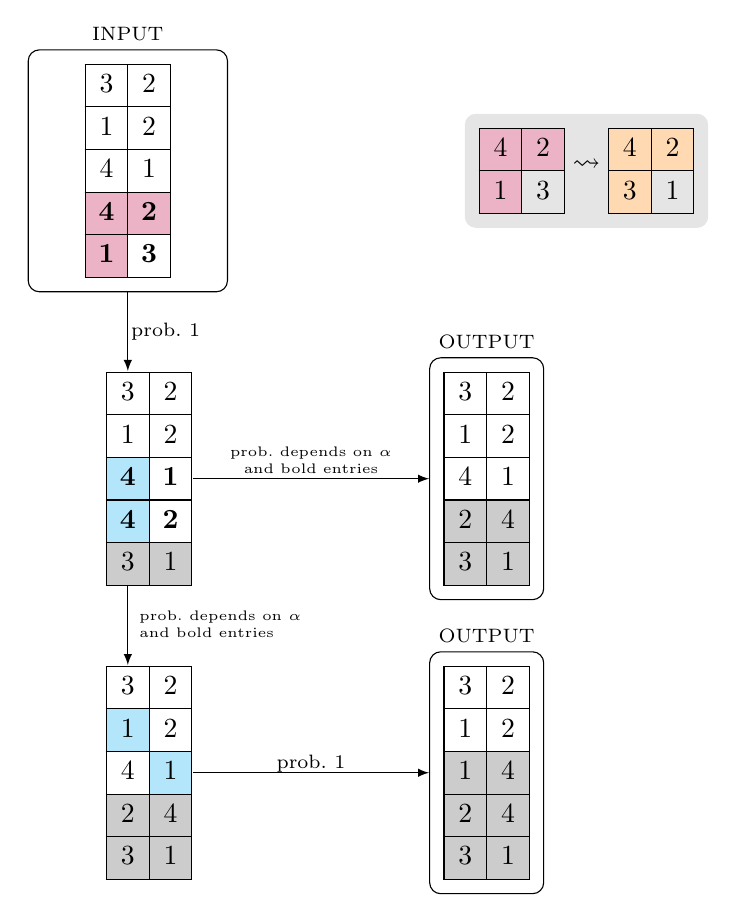
\begin{tikzpicture}[every node/.style={inner sep=0pt}, arrow/.style={-{Stealth[length=2mm]}, thick}]

% Node A (Top-left tableau)
\node[draw, rounded corners, inner sep=5pt, label={[yshift=1mm]above:{\scriptsize INPUT}}] (A) {
  \begin{ytableau}
    \none & 3 & 2 & \none \\
    \none & 1 & 2 & \none \\
    \none & 4 & 1 & \none \\
    \none & *(purple!30) \textbf{4} & *(purple!30) \textbf{2} & \none \\
    \none[\pointer] & *(purple!30) \textbf{1} & \textbf{3} & \none
  \end{ytableau}
};

% Node C (Middle-left tableau)
\uncover<3->{
\node[below=1cm of A] (C) {
  \begin{ytableau}
    \none & 3 & 2 \\
    \none & 1 & 2 \\
    \none & *(cyan!30) \textbf{4} & \textbf{1} \\
    \none[\pointer] & *(cyan!30) \textbf{4} & \textbf{2} \\
    \none & *(gray!40) 3 & *(gray!40) 1
  \end{ytableau}
};
\draw[-latex] (A.south) -- (C.north) node[midway, right=1pt] {\scriptsize prob.\ $1$};
}

% Node D (Middle-right tableau)
\uncover<5->{
\node[right=3cm of C, draw, rounded corners, inner sep=5pt, label={[yshift=1mm]above:{\scriptsize OUTPUT}}] (D) {
  \begin{ytableau}
    3 & 2 \\
    1 & 2 \\
    4 & 1 \\
    *(gray!40) 2 & *(gray!40) 4 \\
    *(gray!40) 3 & *(gray!40) 1
  \end{ytableau}
};
\draw[-latex] (C.east) -- (D.west) node[midway, above] {\tiny\begin{tabular}{c} prob.\ depends on $\alpha$ \\ and bold entries \end{tabular}};
}

% Node E (Bottom-left tableau)
\uncover<6->{
\node[below=1cm of C] (E) {
  \begin{ytableau}
    \none & 3 & 2 \\
    \none & *(cyan!30) 1 & 2 \\
    \none[\pointer] & 4 & *(cyan!30) 1 \\
    \none & *(gray!40) 2 & *(gray!40) 4 \\
    \none & *(gray!40) 3 & *(gray!40) 1
  \end{ytableau}
};
\draw[-latex] (C.south) -- (E.north) node[midway, right=-2pt] {\tiny\begin{tabular}{l}prob.\ depends on $\alpha$ \\ and bold entries \end{tabular}};
}

% Node F (Bottom-right tableau)
\uncover<7->{
\node[right=3cm of E, draw, rounded corners, inner sep=5pt, label={[yshift=1mm]above:{\scriptsize OUTPUT}}] (F) {
  \begin{ytableau}
    3 & 2 \\
    1 & 2 \\
    *(gray!40) 1 & *(gray!40) 4 \\
    *(gray!40) 2 & *(gray!40) 4 \\
    *(gray!40) 3 & *(gray!40) 1
  \end{ytableau}
};
\draw[-latex] (E.east) -- (F.west) node[midway, above] {\scriptsize prob.\ $1$};
}

\uncover<2-3>{
\node[right=3cm of A, fill=gray!20, rounded corners, inner sep=5pt] (S) {
  \(
  \begin{ytableau}
    *(purple!30) 4 & *(purple!30) 2 \\
    *(purple!30) 1 & 3
  \end{ytableau}
  \leadsto
  \begin{ytableau}
    *(orange!30) 4 & *(orange!30) 2 \\
    *(orange!30) 3 & 1
  \end{ytableau}
  \)
};
}
\end{tikzpicture}
\end{frame}

\begin{frame}{All rules about moving the pointer\ \ {\small \faHandPointRight}}
  \centering
	\ytableausetup{smalltableaux}
	\setcellgapes{6pt}
	\makegapedcells
	\begin{tabular}[c]{ccc}
		% \toprule
    % ==== FIRST CASE ====
		\begin{ytableau}
			\none & c & d \\
			\none[\pointer] & a & b \\
      \none & \none[\text{\tiny same inversion type}] 
		\end{ytableau}
		& \(\quad\leadsto \) &
    % ==== FIRST CASE OUTPUT ====
		\begin{ytableau}
			\none & c & d \\
			\none & *(gray!40) b & *(gray!40)a \\
		\end{ytableau}
    \\ % \midrule
    % ==== SECOND CASE ====
		\begin{ytableau}
			\none & c & d \\
			\none[\pointer]   & a & b \\
      \none & \none[\text{\tiny different inversion type}] 
		\end{ytableau}
		& \(\quad\leadsto \) &
    % ==== SECOND CASE OUTPUT ====
		\begin{ytableau}
			\none[\pointer] & c & d \\
			\none & *(gray!40) b & *(gray!40)a \\
		\end{ytableau}
    \\ % \midrule
    % ==== THIRD CASE ====
		\begin{ytableau}
				\none & *(cyan!30) b & d \\
				\none[\pointer]   & a & *(cyan!30) b \\
			\end{ytableau}
		& \(\quad\leadsto \) &
    % ==== THIRD CASE OUTPUT ====
		\begin{ytableau}
			\none & b & d \\
			\none & *(gray!40) b & *(gray!40)a \\
		\end{ytableau}
    \\ % \midrule
    % ==== FOURTH CASE ====
		\begin{ytableau}
				\none & c & *(cyan!30) b \\
				\none[\pointer]   & a & *(cyan!30) b \\
			\end{ytableau}
		& \(\quad\leadsto \) &
    % ==== FOURTH CASE OUTPUT ====
		\begin{ytableau}
			\none[\pointer] & c & b \\
			\none & *(gray!40) b & *(gray!40)a \\
		\end{ytableau}
    \\ % \midrule
    % ==== FIFTH CASE ====
		\begin{ytableau}
				\none & *(cyan!30) a & d \\
				\none[\pointer]   & *(cyan!30) a & b \\
			\end{ytableau}
		& \(\quad\leadsto \) &
		\begin{ytableau}
			\none[\pointer] & a & d \\
			\none & *(gray!40) b & *(gray!40)a \\
		\end{ytableau}
    {\scriptsize or}
		\begin{ytableau}
			a & d \\
			*(gray!40) b & *(gray!40)a \\
		\end{ytableau}
    % ==== FIFTH CASE OUTPUT ====
    \\ % \midrule
    % ==== SIXTH CASE ====
		\begin{ytableau}
				\none & *(cyan!30) a & *(blue!30) b \\
				\none[\pointer]   & *(cyan!30) a & *(blue!30) b \\
			\end{ytableau}
		& \(\quad\leadsto \) &
    % ==== SIXTH CASE OUTPUT ====
		\begin{ytableau}
			\none[\pointer] & a & b \\
			\none & *(gray!40) b & *(gray!40)a \\
		\end{ytableau}
    \\ % \bottomrule
	\end{tabular}
\end{frame}

\begin{frame}{It is a probabilistic bijection!}
  \large

  \begin{theorem}[D--Mandelshtam, 2025\textsuperscript{+}]
    The algorithm describes a probabilistic bijection between
    \(\operatorname{NAF}(\alpha, \sigma)\) and \(\operatorname{NAF}(\alpha, \sigma s_i)\).
  \end{theorem}
  
\end{frame}

\begin{frame}{Thank You}
  \begin{center}
    \ytableausetup{boxsize=1.25em, centertableaux}
    \ytableaushort{TH,ANK,YOU}
    \ \quad
    \(\longleftrightarrow\)
    \quad
    \ytableaushort{TH,ANK,OYU}
  \end{center}
\end{frame}

\appendix

\begin{frame}{\(\alpha = (2, 2, 0, 1)\), \(\sigma = [3, 1, 2, 4]\), content \((1, 2, 0, 2)\)}
  \centering
  \ytableausetup{smalltableaux, centertableaux}
  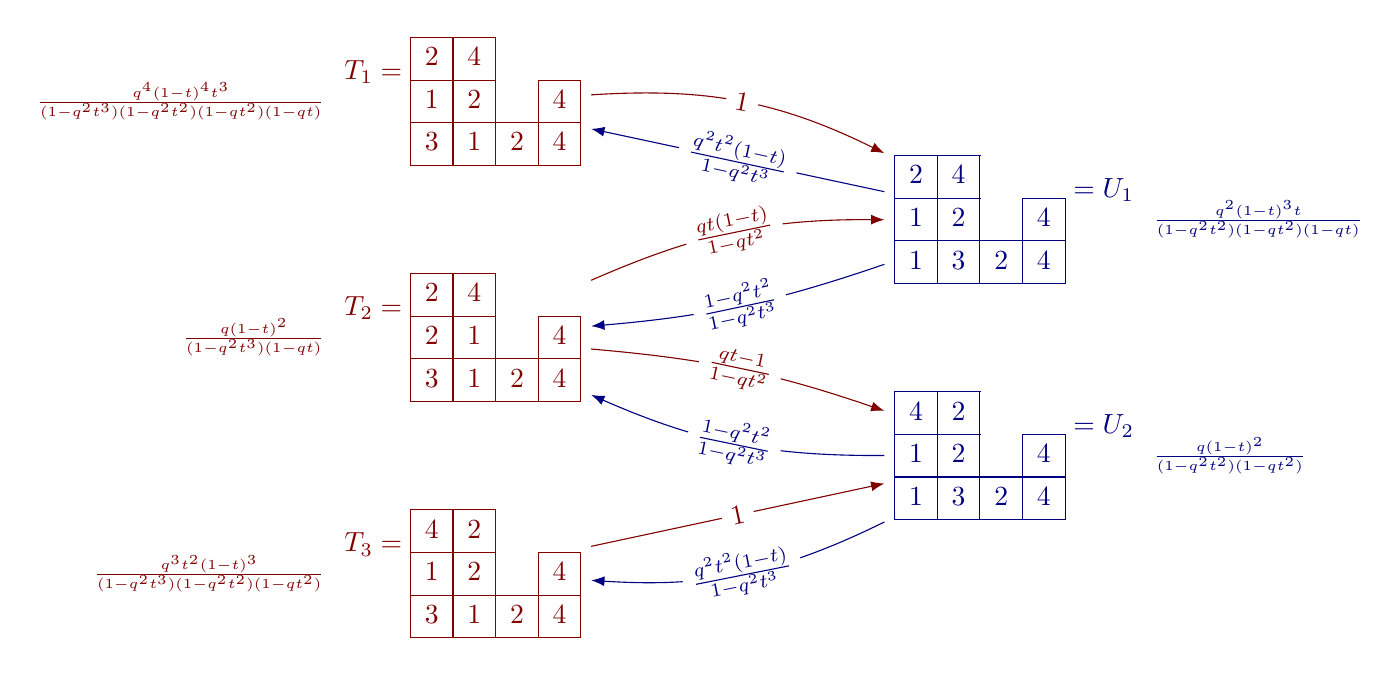
\begin{tikzpicture}
    \node[red!50!black]  (T1) at (-4,  3) {
      $T_1 =
        \begin{ytableau}
          2 & 4 \\
          1 & 2 & \none & 4 \\
          3 & 1 & 2 & 4
        \end{ytableau}$
    };
    \node[red!50!black]  (T2) at (-4,  0) {
      $T_2 =
        \begin{ytableau}
          2 & 4 \\
          2 & 1 & \none & 4 \\
          3 & 1 & 2 & 4
        \end{ytableau}$
    };
    \node[red!50!black]  (T3) at (-4, -3) {
      $T_3 =
        \begin{ytableau}
          4 & 2 \\
          1 & 2 & \none & 4 \\
          3 & 1 & 2 & 4
        \end{ytableau}$
    };
    \node[blue!50!black] (U1) at ( 3,  1.5) {
      $\begin{ytableau}
          2 & 4 \\
          1 & 2 & \none & 4 \\
          1 & 3 & 2 & 4
        \end{ytableau} = U_1$
    };
    \node[blue!50!black] (U2) at ( 3, -1.5) {
      $\begin{ytableau}
          4 & 2 \\
          1 & 2 & \none & 4 \\
          1 & 3 & 2 & 4
        \end{ytableau} = U_2$
    };
    % Weights
    \node[red!50!black, left] at (T1.west) {
      $\scriptstyle \frac{q^{4} {(1 - t)}^{4} t^{3}}{{(1 - q^{2} t^{3})} {(1 - q^{2} t^{2})} {(1 - q t^{2})} {(1 - q t)}}$
    };
    \node[red!50!black, left] at (T2.west) {
      $\scriptstyle \frac{q {(1 - t)}^{2}}{{(1 - q^{2} t^{3})} {(1 - q t)}}$
    };
    \node[red!50!black, left] at (T3.west) {
      $\scriptstyle \frac{q^{3} t^{2} {(1 - t)}^{3} }{{(1 - q^{2} t^{3})} {(1 - q^{2} t^{2})} {(1 - q t^{2})}}$
    };
    \node[blue!50!black, right] at (U1.east) {
      $\scriptstyle \frac{q^{2} {(1 - t)}^{3} t}{{(1 - q^{2} t^{2})} {(1 - q t^{2})} {(1 - q t)}}$
    };
    \node[blue!50!black, right] at (U2.east) {
      $\scriptstyle \frac{q {(1 - t)}^{2}}{{(1 - q^{2} t^{2})} {(1 - q t^{2})}}$
    };
    % Arrows
    \draw[-{Latex}, red!50!black]  (T1) edge[bend left=15] node[sloped, fill=white]{\(1\)} (U1);
    \draw[-{Latex}, blue!50!black] (U1) edge[bend left=0] node[sloped, fill=white]{\(\tfrac{q^2t^2(1-t)}{1-q^2t^3}\)} (T1);
    \draw[-{Latex}, red!50!black]  (T2) edge[bend left=12] node[sloped, fill=white]{\(\frac{qt(1-t)}{1-qt^2}\)} (U1);
    \draw[-{Latex}, blue!50!black] (U1) edge[bend left=7] node[sloped, fill=white]{\(\frac{1-q^2t^2}{1-q^2t^3}\)} (T2);
    \draw[-{Latex}, red!50!black]  (T2) edge[bend left=7] node[sloped, fill=white]{\(\frac{qt-1}{1-qt^2}\)} (U2);
    \draw[-{Latex}, blue!50!black] (U2) edge[bend left=12] node[sloped, fill=white]{\(\frac{1-q^2t^2}{1-q^2t^3}\)} (T2);
    \draw[-{Latex}, red!50!black]  (T3) edge[bend left=0] node[sloped, fill=white]{\(1\)} (U2);
    \draw[-{Latex}, blue!50!black] (U2) edge[bend left=15] node[sloped, fill=white]{\(\tfrac{q^2t^2(1-t)}{1-q^2t^3}\)} (T3);
  \end{tikzpicture}
\end{frame}

\newcommand{\twinv}{\operatorname{twinv}} % Define the \twinv command

\begin{frame}{Future Work: \(\alpha_i \neq \alpha_{i+1}\) via probabilistic bijections}

If \(\alpha_i < \alpha_{i+1}\) and \(\sigma_i > \sigma_{i+1}\), then
\[
  %\setlength{\thickmuskip}{20mu}
  %\setlength{\medmuskip}{15mu}
  \textcolor{red!70!black}{E_{s_i\alpha}^\sigma(X;q;t)}
  =
  \textcolor{red!70!black}{E_{\alpha}^{\sigma s_i}(X;q;t)}
  +
  \tfrac{t^{\phi(\alpha,\sigma,i)}(1-t)}{1-q^{L+1}t^{A}}
  \textcolor{red!70!black}{E_{\alpha}^\sigma(X;q;t)}
\]
{\small where $A=\arm(x)$ and $L=\leg(x)$ for $x=(i+1,\alpha_i+1)\in\dg(\alpha)$.}
\end{frame}

\begin{frame}{Idea for Proof of Balance Condition}
  \begin{itemize} \itemsep .5em
    \item Define the component of the weight contributed by the row \(r\) such that
    \begin{equation*}
      \wtqt(T) = \prod_{\text{row } r} \wtqt^{(r)}(T).
    \end{equation*}
    \item Define the probability that the pointer moves up in row \(r\) denoted by \(\rho^{(r)}(T)\).
    \item Prove ``balance condition'' row-by-row:
    \begin{align*}
      \wtqt^{(r)}(T) \cdot \rho^{(r)}(T) &= \wtqt^{(r)}(U) \cdot \rho^{(r)}(U) \qquad \text{or} \\
      \wtqt^{(r)}(T) \cdot \left( 1 - \rho^{(r)}(T) \right) &= \wtqt^{(r)}(U) \cdot \left( 1 - \rho^{(r)}(U) \right),
    \end{align*}
    with the appropriate choice of \(\rho\) (move pointer up) or \(1 - \rho\) (delete).
  \end{itemize}
\end{frame}

\begin{frame}{References}
  \AtNextBibliography{\small}
  \printbibliography
\end{frame}

\end{document}
